\chapter{Results: Online Sources}\chlbl{online_sources}
%
\begin{figure}[h]
    \centering
    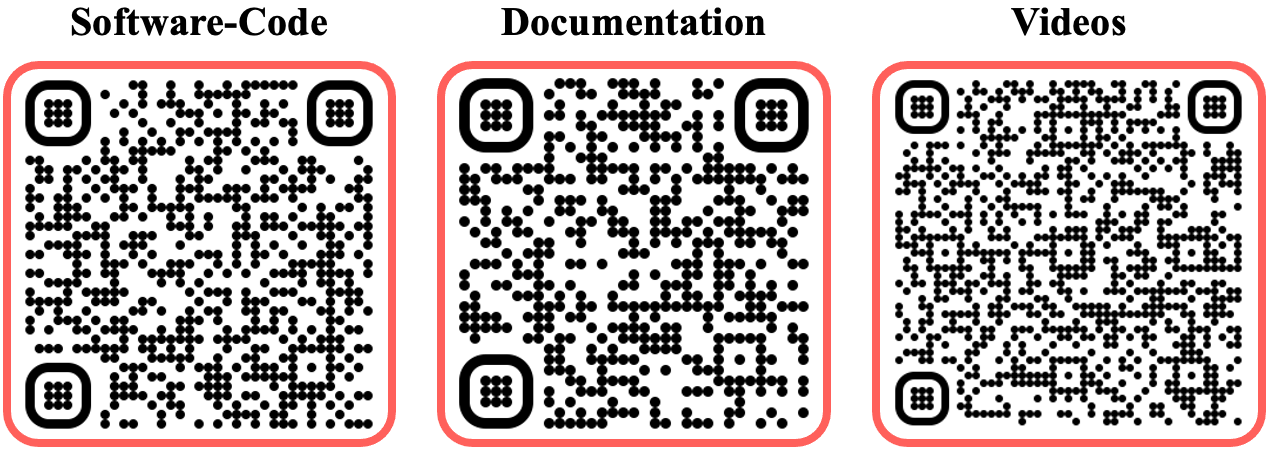
\includegraphics[width=0.79\textwidth]{qr_links}
    \caption[QR-Codes with links to sources]{QR-Codes with links to sources. The first code directs to the Github repository containing the source code, the second code to the repository containing the \LaTeX files to build this documentation, and the third code points to video visualisations of the results.}
    \figlbl{qr_links}
\end{figure}
%
The code and results from this thesis  have been made available as open source on Github: The code is available at \url{https://github.com/sagerpascal/lateral-connections}, and the documentation is available at \url{https://github.com/sagerpascal/msc-thesis}.
Furthermore, a Github webpage provides video visualisations from some of the results at \url{https://sagerpascal.github.io/lateral-connections/results/final_results.html}.
\figref{qr_links} makes these links available as QR codes so that they can easily be accessed with electronic devices.

\section{Video}\chlbl{result_video}
%
\begin{figure}[h]
    \centering
    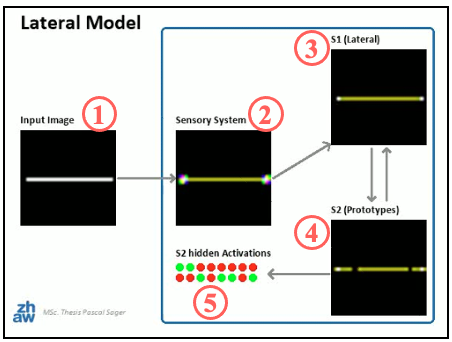
\includegraphics[width=0.99\textwidth]{video_overview}
    \caption[Overview of components visualised in the videos]{An overview of the components visualised in the videos.}
    \figlbl{video_overview}
\end{figure}
%
In the following, the video visualisations accessible at \url{https://sagerpascal.github.io/lateral-connections/results/final_results.html} are explained.
However, the explanations are limited to an overview of which components are shown in each video.
A specific interpretation of the video content is provided in the corresponding result section.

Two video versions are shown for each experiment, both produced by the same model using the same parameter weights.
In the first video version, the Bernoulli neuron is replaced by a neuron using a fixed threshold.
This provides a video output that is more stable and has no flickering activations caused by sampling from a probability distribution.
For the \emph{S0} and \emph{S1} stages, a threshold of $0.5$ is used. Consequently, neurons with a probability of $\geq 0.5$ are set to $1$, while the other neurons are set to $0$.
For the \emph{S2} stage, a threshold of $0.9$ is used, visualising only activities with high certainty that roughly correspond to those accepted by \emph{S1} as feedback signals.
The second video shows the network activities when the Bernoulli neurons are used.

Each video visualises the processing of the input over time.
The first six video frames show how the video is processed over the $T=6$ timesteps of the fast loop, followed by five additional frames depicting the final prediction after the fast loop.
By doing so, viewers have time to analyse the network's activations during this short interruption before the next input is fed into the model and the process repeats.

\figref{video_overview} shows a single video frame, providing an overview of the components displayed in each video:
\begin{enumerate}
    \item The left part of the video displays the input image fed into the sensory system. It is a binary image with one colour channel, whereby active pixels are depicted in white and inactive pixels are depicted in black.
    \item The activations of the sensory system are shown in the middle of the video. The sensory system extracts $4$ features at each location. Each feature combination is visualised in a different colour, and locations without any activations are depicted in black.
    \item \emph{S1} is visualised in the top right corner. It uses the same colours as the sensory system. However, the activations might differ since neurons with insufficient lateral support are turned off.
    \item \emph{S2} is shown in the bottom right corner. It uses the same colours as the sensory system and \emph{L1}. The visualisation depicts the reconstructed version, i.e., the feedback provided to \emph{S1} after mapping \emph{S1}' activities to the latent variables.
    \item The latent variables of \emph{S2} are shown at the center bottom of the video as $16$ circles. Each circle represents a cell, with green indicating an active cell and red indicating an inactive one. 
\end{enumerate}

For a detailed explanation of the content and observations in each video, please refer to the results chapter of this thesis.




\chapter{Negative Hebbian Learning}\chlbl{neg_hebb_updates}
%
\begin{figure}[h]
    \centering
    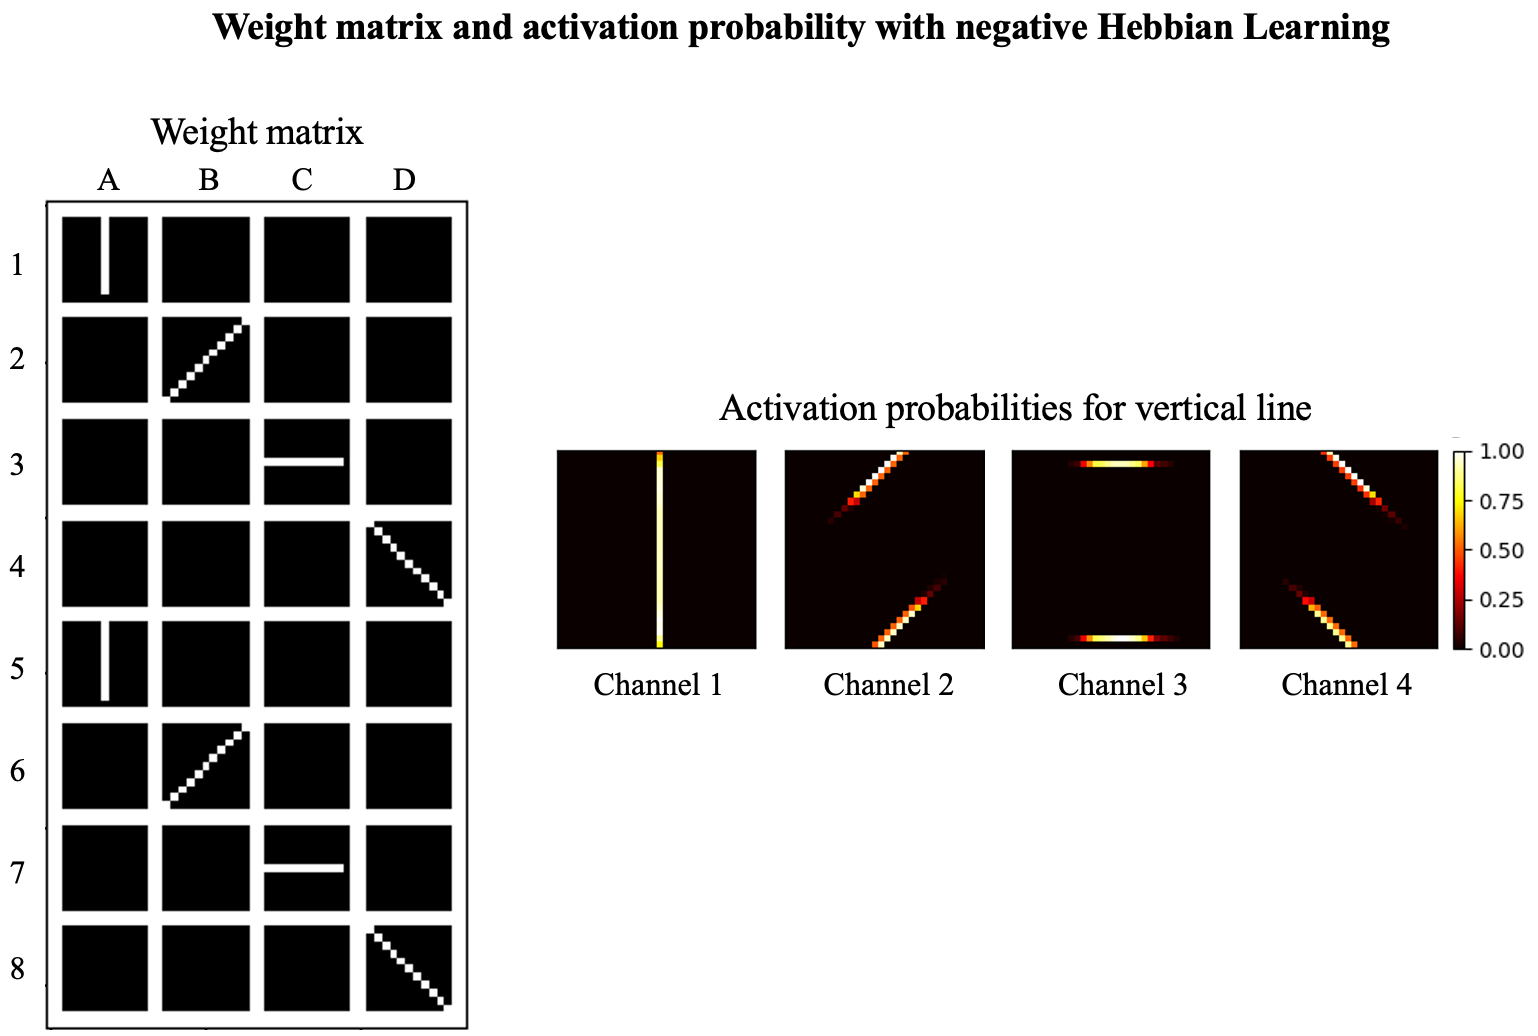
\includegraphics[width=0.99\textwidth]{neg_hebb_learning}
    \caption[Weight matrix and activations with negative Hebbian learning]{The weight matrix and the corresponding activation probabilities for a vertical line of a model trained with negative Hebbian learning.}
    \figlbl{neg_hebb_learning}
\end{figure}
%
This section examines the concept of negative Hebbian Learning in \emph{S1}, a learning mechanism designed to enable neural networks to forget unimportant or incorrect features. 
So far, only positive Hebbian learning is used to strengthen connections between active cells.
Negative Hebbian learning additionally reduces the connection strength between cells that fire disjointly.
While negative Hebbian learning allows to eliminate previously learned connections, it also presents challenges in maintaining supportive relationships between distinct features.

\figref{neg_hebb_learning} visualises the weight matrix and the activation probabilities for a vertical line fed into a model trained with negative Hebbian learning.
Even tough the activations probabilities look different than for positive Hebbian learning, they are still considered valid representations of lines.
However, the main issue is that the output channels do not rely on distinct features.
For example, the output channel $A$ representing vertical lines only considers the input channels $1$ and $5$, whereby channel $1$ contains the ``vertical lines features'' from the sensory system and channel $5$ is the recurrent connection.
However, the other sensory signals, arriving at input channel $2$-$4$ are not taken into account by output channel $A$.
Thus, only cells representing vertical line features support this output channel.
In contrast, positive Hebbian learning considers all input channels.


Therefore, the lateral support is lower with negative Hebbian learning.
This might not be an issue for the used line dataset but is crucial for real world scenarios\sidenote{For example, a channel could represent eyes and another eyelashes. These features should support each other.}.
Thus, negative Hebbian learning can forget irrelevant features, but also suffers from features becoming mutually exclusive, which prevents adequate support between them.

\begin{figure}[h]
    \centering
    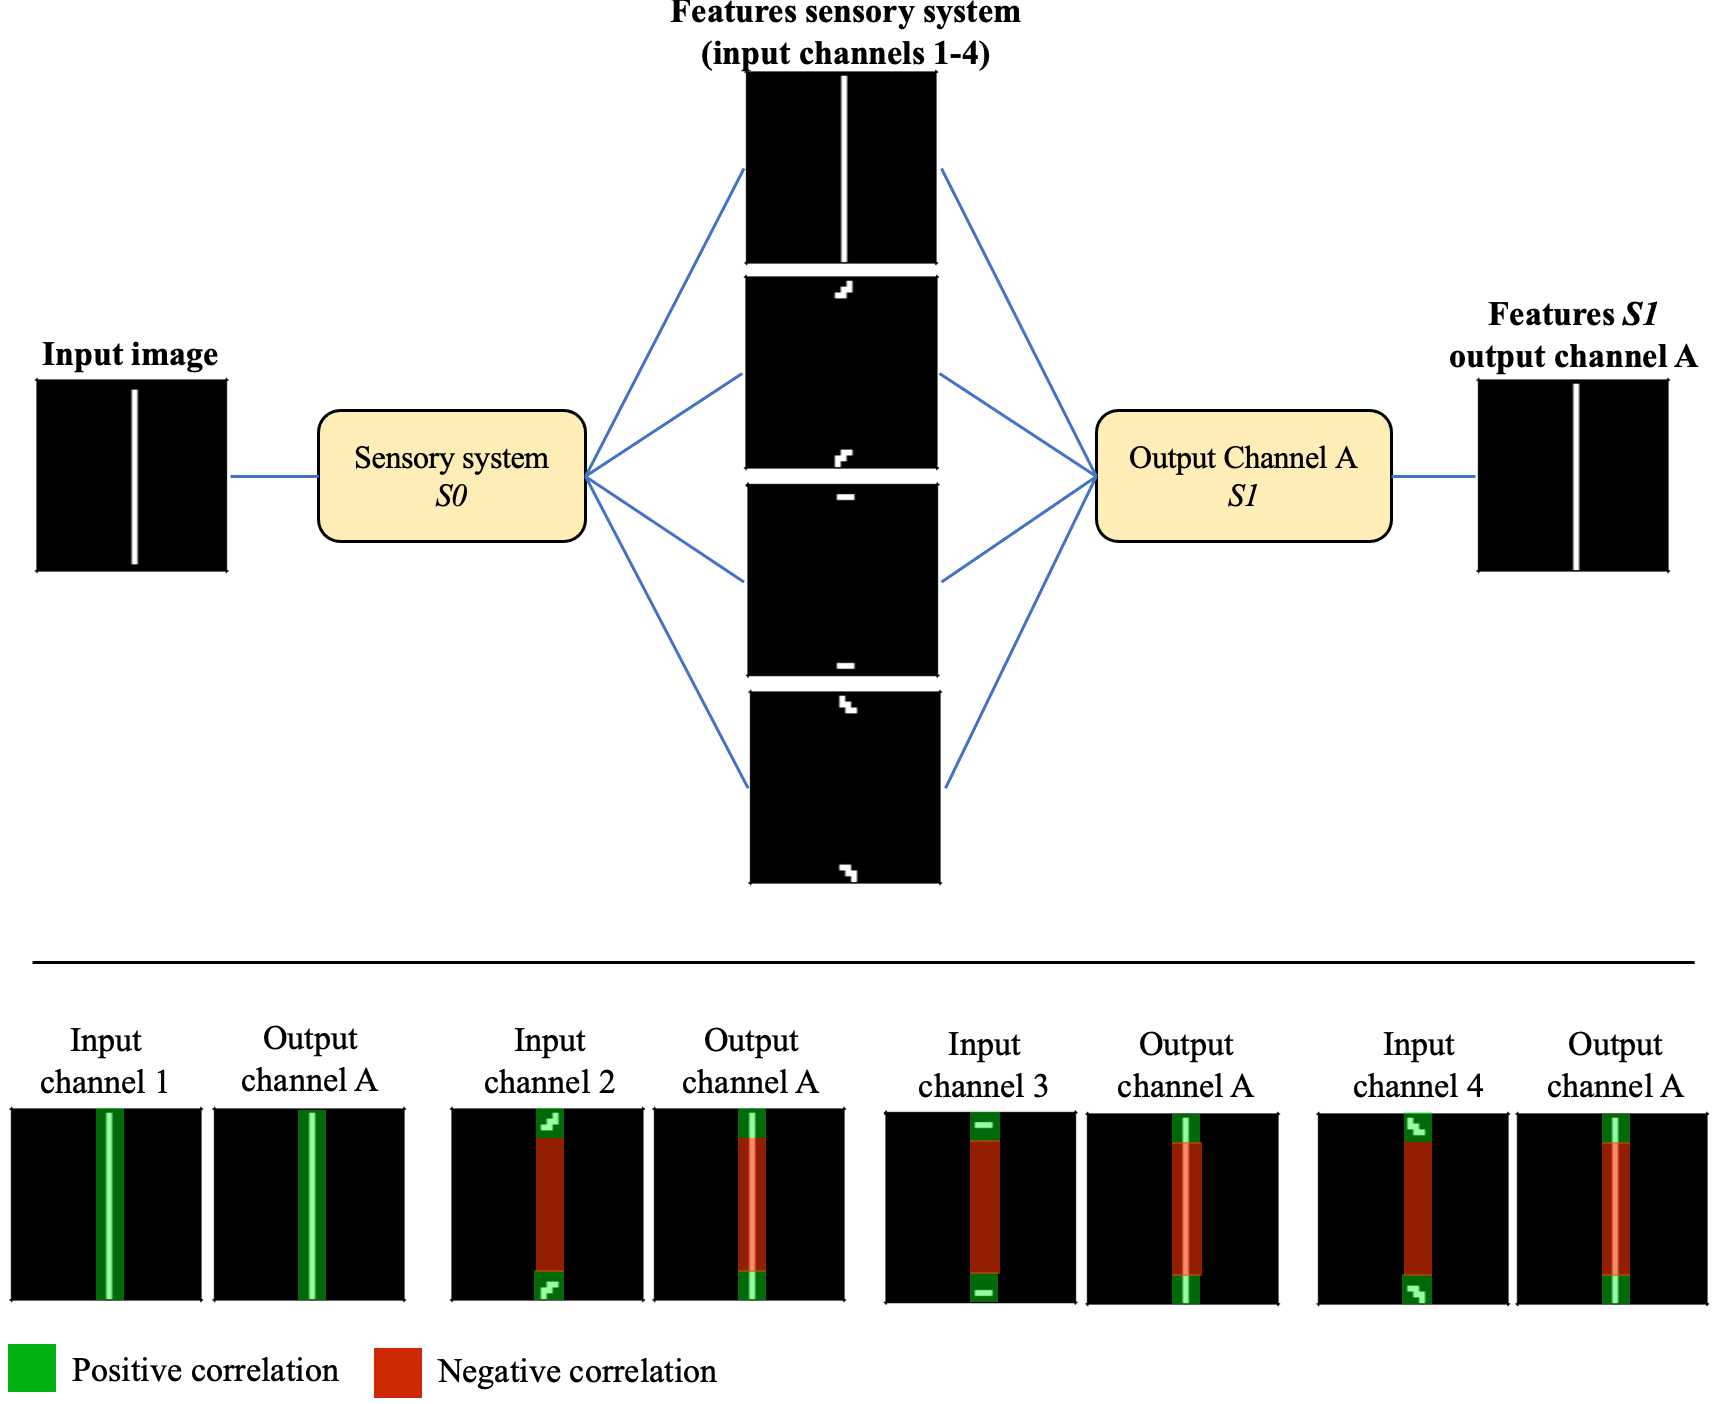
\includegraphics[width=0.99\textwidth]{correlations_hebb_learning}
    \caption[Feature correlations]{Correlation between features from the input channels and the output channel $A$. The upper part of the images visualises the features fed into channel $A$ and the expected result. The lower part of the image indicates where positive and negative correlation occurs between input channels and output channel $A$.}
    \figlbl{correlations_hebb_learning}
\end{figure}
%
In the following, it is discussed why the features become mutually exclusive.
The primary issue is that, except for one input channel, there is more negative correlation between the input channels and a single output channel, as visualised in \figref{correlations_hebb_learning}.
In this context, ``negative correlation'' refers to disjointly active cells while ``positive correlation'' refers to cells that fire together.
In the case of the vertical line, it is expected that output channel $A$ roughly reassembles the line.
Hebbian learning compares this output to the input channels and increases the weight if there is a positive correlation between input and output and decreases the weight if the correlation is negative.
These correlations are visualised in the lower part of \figref{correlations_hebb_learning}.
Input channel $1$ and output channel $A$ are roughly identical, therefore, the activations between input and output have a positive correlation and the corresponding lateral connections undergoes a positive Hebbian update.

However, all the other channels have only at the line ends a positive correlation, and a negative correlation in the middle section of the line.
Therefore, there is more negative correlation than positive correlation and these features undergo more negative updates than positive updates.

The resolution to this issue remains unclear and require additional experiments. One potential approach is to use a significantly smaller learning rate for negative updates than for positive updates, another solution could be to introduce alternative cells (c.f. \secref{TODO})

